\documentclass[a4paper,10pt]{article}
\usepackage[margin=0.53in]{geometry}
\usepackage{graphicx}
\usepackage{array}
\usepackage{enumitem}
\usepackage{titlesec}
\usepackage{setspace}
\usepackage{multicol}
\usepackage{ragged2e}
\usepackage[none]{hyphenat}
\usepackage{qrcode}
\renewcommand{\baselinestretch}{1.1}
\setlength{\parindent}{0pt}
\pagestyle{empty}

% Supervisor designation: replace with the exact title (Assistant / Associate Professor)
\newcommand{\supdesig}{Associate Professor}

\begin{document}
\centering
\begin{tabular}{|l@{\hspace{1em}}|>{\raggedright\arraybackslash}p{12cm}|}

\hline
\multicolumn{2}{|p{18cm}|}{
\centering \textbf{Multilingual Sentiment \& Need Detection from Social Media for Real-Time Crisis Monitoring and Departmental Routing}
\vspace{0.15cm}
} \\
\hline
\multicolumn{2}{|p{16cm}|}{
\textbf{Domain:} Natural Language Processing, Machine Learning, Crisis Informatics
\vspace{0.1cm}
} \\
\hline
\multicolumn{2}{|p{18cm}|}{
\textbf{Abstract:}\newline
\justifying
During crises, people post information, emotions and requests for help on social media in many languages, often code-mixed or romanized. Existing tools are largely English-only, analyse sentiment without detecting actual needs, cannot separate credible reports from rumours, and do not route anything to the departments that must act. This project builds a real-time multilingual pipeline that turns a stream of posts into verified, prioritised alerts for government departments. Posts in English, Hindi, Kannada, Tamil and Telugu are cleaned, de-duplicated and language-tagged, filtered by a fine-tuned disaster classifier (89\% test accuracy), and analysed for sentiment and department-specific needs (93\% test accuracy for need detection). IndicSBERT embeddings group reports of the same event into clusters, and each cluster is scored for priority (severity, actionability, corroboration, credibility, recency) and fake-news risk (content risk, low credibility and copy-paste amplification). Every situation carries a template-based summary in five languages and ranked, privacy-masked evidence posts. A human reviewer approves, rejects or marks each situation fake; approved situations are routed as tickets to every department whose need is detected, and urgent situations left unreviewed are auto-escalated as unverified. An analytics dashboard shows live trends, department and language heatmaps, response times and stored daily situation reports.
} \\
\hline
\multicolumn{2}{|p{16cm}|}{
\begin{minipage}[t]{\linewidth}
\textbf{Architecture / Flow Diagram:}

\vspace{6pt}
\end{minipage}
} \\
\multicolumn{2}{|c|}{
  \begin{minipage}{\linewidth}
    \centering
    % High-level design (docs/HLD.png), full box width
    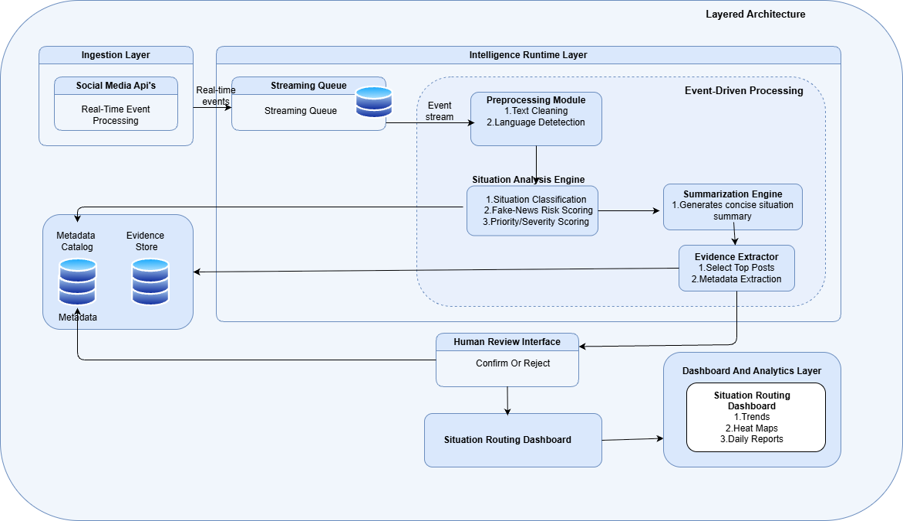
\includegraphics[width=17cm]{160_1.png}
    \vspace{10pt}
  \end{minipage}
} \\

\hline
\begin{tabular}[t]{@{}l@{}}
\textbf{Supervisor:} \\[0.8ex]
Dr. Saritha \\[-0.1em]
\small \supdesig
\end{tabular}
&
\begin{tabular}[t]{@{}l@{}}
\textbf{Team No.:} 160 \\[0.8ex]
\begin{tabular}[t]{@{}l@{\hspace{5pt}}l@{\hspace{5pt}}l@{\hspace{5pt}}l@{}}
\small\textbf{Akshata Udaganve} & \small\textbf{Christananda B} & \small\textbf{Devraj Ishwar Naik} & \small\textbf{Favaz Ahmed Alam} \\
\small PES2UG23CS043 & \small PES2UG23CS158 & \small PES2UG23CS167 & \small PES2UG23CS190 \\
\end{tabular}
\end{tabular} \\
\hline

% Paper not yet published: space left empty, QR code removed.
\multicolumn{2}{|p{16cm}|}{
\textbf{Publication:}
} \\
\multicolumn{2}{|p{18cm}|}{
  \rule{0pt}{2.5cm}
} \\

\hline
\end{tabular}

\end{document}
